\begin{frame}
\frametitle{Invertierender Verstärker}
\framesubtitle{}
    \begin{block}{Invertierender Verstärker}
        \begin{itemize}
                \item $U_{in}$ liegt auf invertierendem Eingang
                \item $U_{out}$ Rückgekoppelt mit $U_{in}$.
                \item Goldene Regel: OPV wird versuchen $U_{out}$ so auszugeben
                dass Eingangsdifferenz $=0$
        \end{itemize}
    \end{block}
            \begin{figure}[H]
            \begin{center}
                    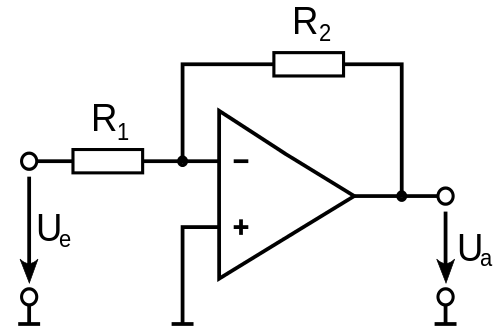
\includegraphics[scale=0.2]{./img/schaltung/inv_verst_0.png}
            \end{center}
            \end{figure}
\end{frame}

\begin{frame}
\frametitle{Invertierender Verstärker}
\framesubtitle{}
    \begin{columns}[c]
        \column{0.8\textwidth}
            \begin{block}{Technische Funktionsweise:}
                \begin{itemize}
                    \item OPV gibt Spannung $U_{R_2}$ so aus dass $U_{diff} =0$:
                        \begin{equation*}
                            U_a = -U_{R_1}
                        \end{equation*}
                    \item Da $I_- = 0$, muss $I_{R_1} = I_{R_2}=I$:
                        \begin{equation*}
                            U_a = -U_{R_1} = -I \cdot R_2 = - \frac{U_e}{R_1}
                            \cdot
                            R_2 = -\frac{R_2}{R_1} \cdot U_e
                        \end{equation*}
                    \item Also gilt für die Verstärkung:
                        \begin{equation*}
                            V = \frac{U_a}{U_e} = - \frac{R_2}{R_1}
                        \end{equation*}
                \end{itemize}
            \end{block}
        \column{0.3\textwidth}
            \begin{figure}[H]
            \begin{center}
                    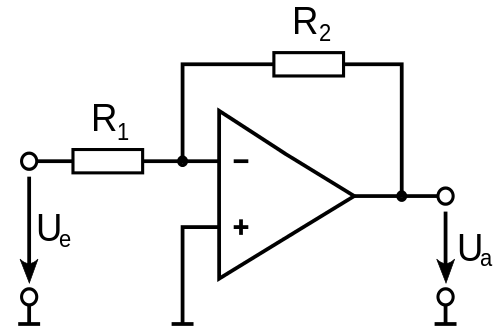
\includegraphics[scale=0.1]{./img/schaltung/inv_verst_0.png}
            \end{center}
            \end{figure}
    \end{columns}
\end{frame}

\begin{frame}
\frametitle{Versuchsaufbau}
\framesubtitle{}
    \begin{block}{Versuch}
        \begin{itemize}
            \item Aufbau wurde mit Batteriespannung $\pm 9V$ betrieben
            \item Bestimmung der Spannungsverstärkung
        \end{itemize}    
    \end{block}    
    \begin{figure}[H]
    \begin{center}
            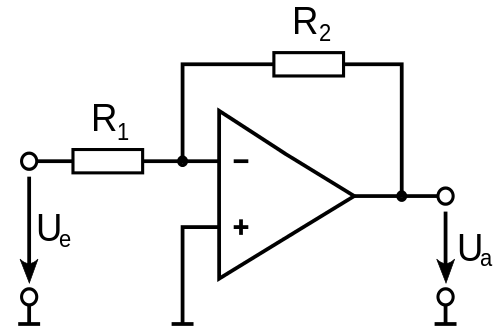
\includegraphics[scale=0.2]{./img/schaltung/inv_verst_0.png}
    \end{center}
    \end{figure}
\end{frame}

\begin{frame}
\frametitle{Bestimmung der Verstärkung}
\framesubtitle{}
    \begin{columns}[c]
    \column{0.6\textwidth}
        \begin{block}{Verstärkung}
            \begin{itemize}
                \item Theoretischer Wert:
                    \begin{equation*}
                        V=-\frac{R_2}{R_1} = -\frac{-47k\Omega}{10k\Omega}=-4.7
                    \end{equation*}
                \item Ermittelter Wert (Fit):
                    \begin{equation*}
                        V=-4.65    
                    \end{equation*}
            \end{itemize}
        \end{block}
    \column{0.4\textwidth}
        \begin{figure}[H]
        \begin{center}
                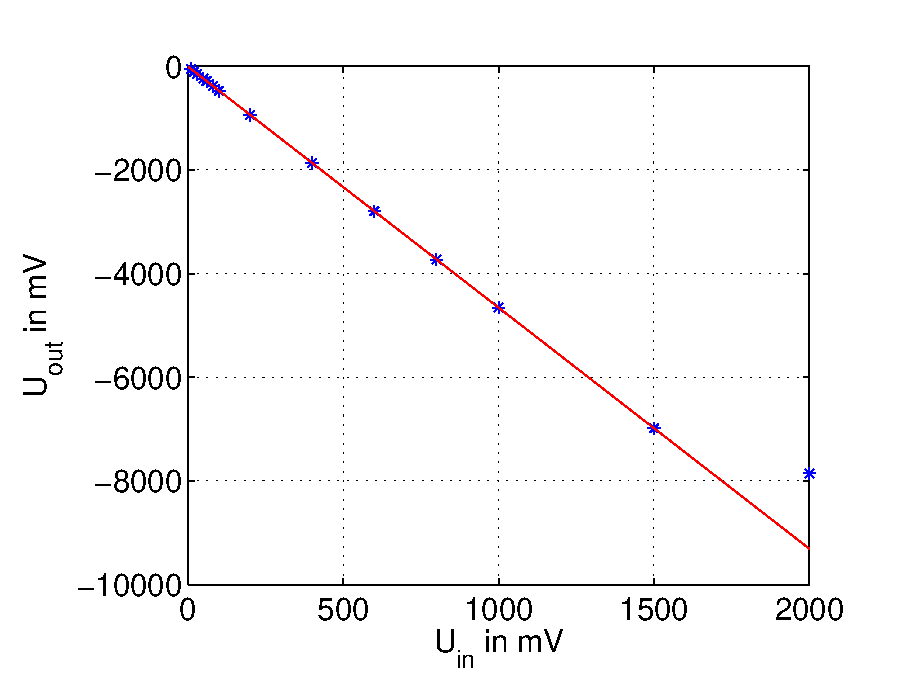
\includegraphics[scale=0.35]{./img/plots/Auf_2_Uout_Uin.eps}
        \end{center}
        \end{figure}
    \end{columns}
\end{frame}

\begin{frame}
\frametitle{Bodediagramm}
\framesubtitle{}
    \begin{columns}[c]
    \column{0.5\textwidth}
        \begin{figure}[H]
        \begin{center}
                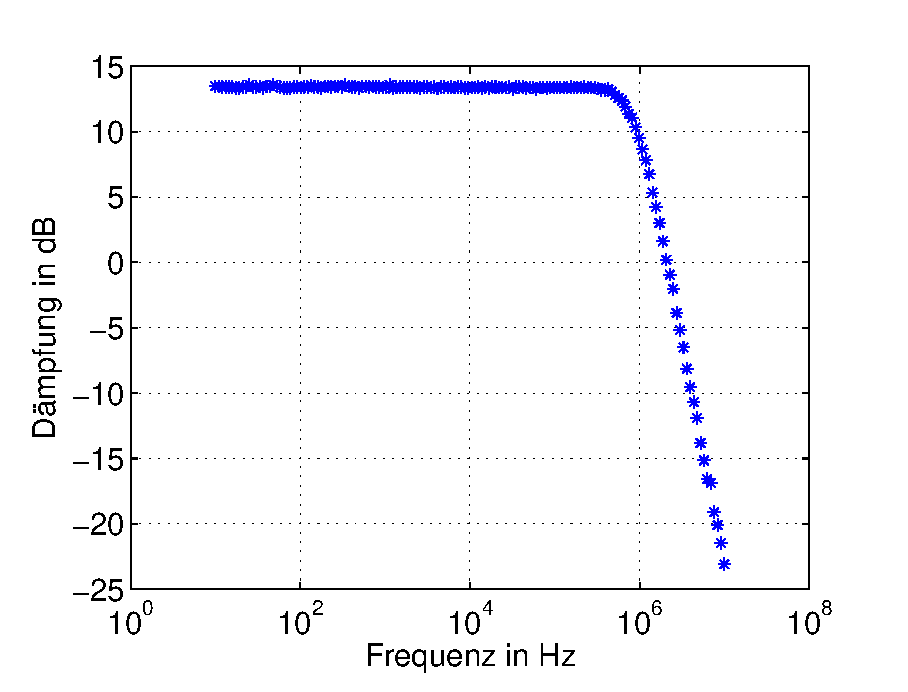
\includegraphics[scale=0.4]{./img/plots/Auf_2_bode_db.eps}
        \end{center}
        \end{figure}
    \column{0.5\textwidth}
        \begin{figure}[H]
        \begin{center}
                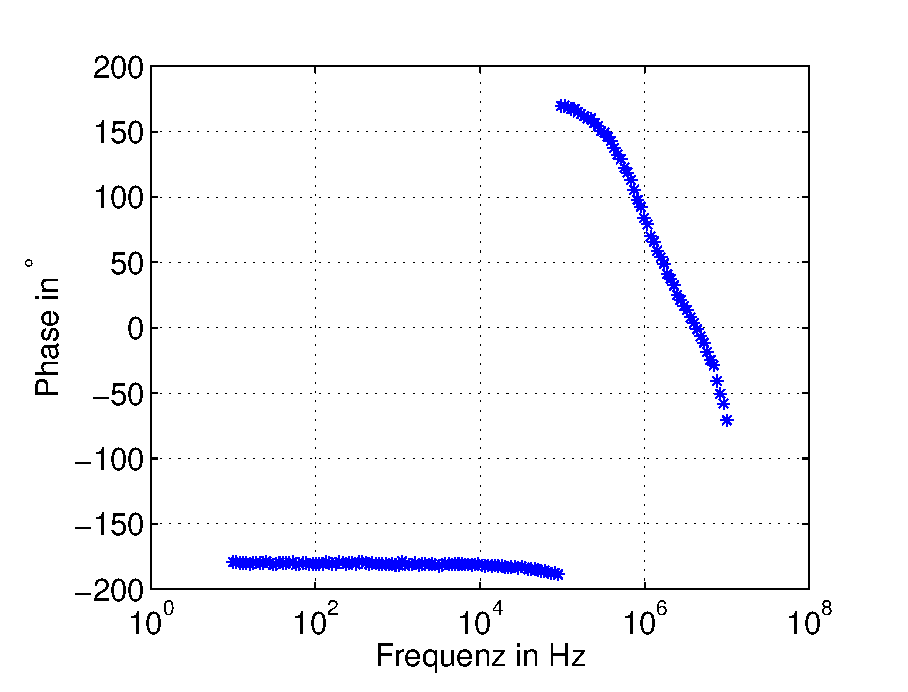
\includegraphics[scale=0.4]{./img/plots/Auf_2_bode_ph.eps}
        \end{center}
        \end{figure}
    \end{columns}
    \begin{block}{}
        \begin{itemize}
            \item Hohe Verstärkung bei niedrigen Frequenzen: 
            \item Zusammenbruch bei hohen Frequenzen: Tiefpass mit
            $3dB$-Frequenz: $690kHz$
            Messgeräten
        \end{itemize}
    \end{block}
\end{frame}

\begin{frame}
\frametitle{Versuchsaufbau mit Kondensator}
\framesubtitle{}
    \begin{block}{Versuch}
        \begin{itemize}
            \item Aufbau wurde mit Batteriespannung $\pm 9V$ betrieben
            \item Setze $R_6 = 1M\Omega$
            \item Einbau von Kondensator $C_5 = 22\mu F$ vor $R_5$
        \end{itemize}    
    \end{block}    
    \begin{block}{Theoriewerte:}
    \begin{itemize}
        \item für Impedanz an $R_5$ gilt:
            \begin{equation*}
                R_5 \rightarrow R_5 + \frac{1}{i \omega \cdot C}    
            \end{equation*}
        \item also folgt für Verstärkung:
            \begin{equation*}
                V = \frac{R_6}{R_5 + \omega \cdot C}
            \end{equation*}
    \end{itemize}
    \end{block}
\end{frame}

\begin{frame}
\frametitle{Verstärkung mit Kondensator}
\framesubtitle{}
    \begin{columns}[c]
    \column{0.6\textwidth}
        \begin{block}{Messung}
        \begin{itemize}
            \item Aus Theorie folgt mit
            $\omega=800mHz$,$R_2=1M\Omega$,$R_1=10k\Omega$,$C=22\mu F$:
            \begin{equation*}
                V = -99.9
            \end{equation*}
            \item Mit $A_2 = 3.75 V$ und $A_1=49.1mV$ tatsächliche Verstärkung:
            \begin{equation*}
                V = \frac{A_2}{A_1} \approx -83.3
            \end{equation*}
            \item DC-Offset wird fast vollständig herausgefiltert
            \item Phasenverschiebung um $\sim 143^{\circ}$
        \end{itemize}
        \end{block}
    \column{0.5\textwidth}
    \begin{figure}[H]
    \begin{center}
            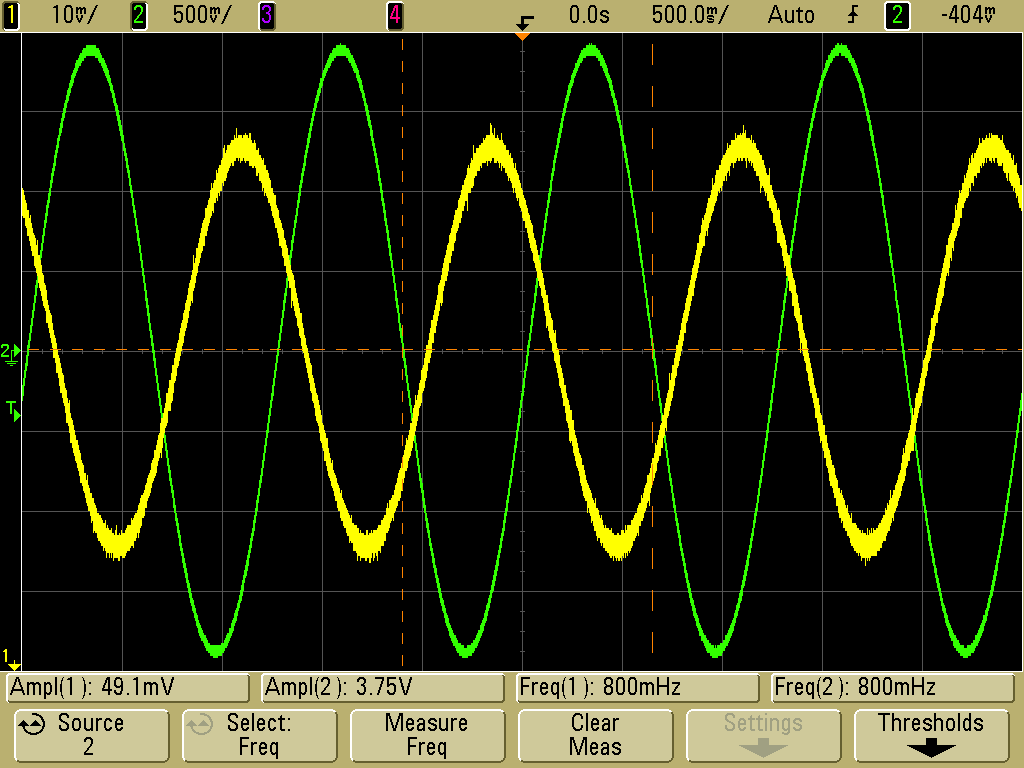
\includegraphics[scale=0.15]{./img/oszi/scope_2.png}
    \end{center}
    \end{figure}
    \end{columns}
\end{frame}

\begin{frame}
\frametitle{Erbenisse}
\framesubtitle{}
\begin{block}{Ergebnisse}
     \begin{itemize}
         \item höherer Widerstand $R_6$ verbessert Verstärkung
         \item Kondensator filter Offset heraus
         \item Potential an invertierendem Eingang wird "virtuell" genannt da
         dort ein Massepotenzial ohne Verbindung zur Masse anliegt
     \end{itemize}
\end{block}
\end{frame}
